\section{Elektronik}

\subsection{Messwertverarbeitung}
Die Messwertverarbeitung findet direkt auf dem Mikrokontroller statt.

\subsection{Leistungsteil}
Als Leistungsteil soll ein Step-Up-Modul die Spannung des 4S-LiPo’s auf 24V hoch transformieren, um die Motoren mit der maximal verträglichen Spannung zu versorgen. 

\begin{figure}[H]
    \begin{center}
    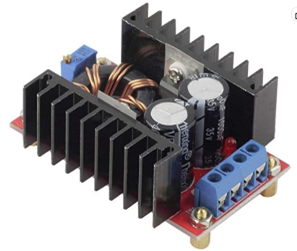
\includegraphics[width=6.3cm]{Elektronik_StepUp.png}
    \end{center}
    \caption{Step-Up}
\end{figure}

Des Weiteren soll auch ein Step-Down Modul zum Einsatz kommen, um die 5V Versorgerspannung für den Microkontroller bereitzustellen. 

\begin{figure}[H]
    \begin{center}
    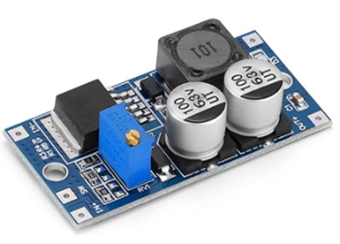
\includegraphics[width=6.3cm]{Elektronik_StepDown.png}
    \end{center}
    \caption{Step-Down}
\end{figure}

Da die Kühlbox auf die Nennspannung einer Autobatterie ausgelegt war, welche durchschnittlich 12-14V liefert, haben wir von einer weiteren Spannungstransformation abgesehen und die Kühlbox mit der Batteriespannung versorgt.
